\subsection{\label{subsec:A1}Röntgenstrahlabsorption}
\subsubsection{Kalibrierung}
Um die Messergebnisse, deren Gewinnung in Abschnitt 
\ref{subsec:vers1} beschrieben ist, nutzbar zu machen, muss zunächst 
der gemessene Beugungswinkel $\Theta$ mit der gebeugten Wellenlänge $\lambda$ 
in Verbindung gebracht werden. Hierzu verwenden wir die Braggsche 
Gleichung \eqref{eq:bragg} und die Berechnung des Netzebenenabstands, für 
welchen im kubischen System folgendes gilt
\begin{equation}
    d_{hkl} = \frac{a}{\sqrt{h^{2} + k^{2} + l^{2}}}.
\end{equation}
Da der Kristall so präpariert wurde, dass der Röntgenstrahl an der (220)-Ebene gebeugt wird,
folgt
\begin{align}
    d_{220} &\coloneqq d = \frac{a}{\sqrt{2^{2} + 2^{2} + 0^{2}}} \approx 1,931462\,\si{\angstrom} \\
    s_{d} &= \frac{s_{a}}{\sqrt{8}} \approx 0,000354\,\si{\angstrom} \\
    \Rightarrow \Aboxed{d &= (1,9315 \pm 0,0004)\,\si{\angstrom}}.
\end{align}
Der berechnete Fehler $s_{d}$ ist so gering, dass er für die weitere Berechnung keine Rolle spielt. \\
Aus Gl.~\eqref{eq:bragg} folgt 
\begin{align}
    \lambda &= \frac{2d}{n}\sin(\Theta)  \label{eq:welle} \\
    \Leftrightarrow \Theta &= \arcsin\left(\frac{n\lambda}{2d}\right), \label{eq:winkel}
\end{align}
womit wir die gemessenen Winkel in Wellenlängen und zurück rechnen können. \\
Weiterhin muss eine Winkelkalibrierung erfolgen, die den gemessenen Winkel mithilfe
theoretischer Referenzpunkte mit einem realen Winkel in Verbindung bringt. 
Bei einer idealen Justierung und einem perfekten Messaufbau könnte auf diesen Schritt 
verzichtet werden, hier aufgrund der benötigten Genauigkeit jedoch durchgeführt.
Die Referenzpunkte sind durch die charakteristische Röntgenstrahlung der Wolfram-Anode 
gegeben, wobei Tabelle 1 der Versuchsanleitung \cite{Anleitung} die erlaubten 
Übergänge auflistet. Rechnet man die theoretische Lage über Gl.~\eqref{eq:winkel} 
in Winkel um, an denen die Linien erwartet werden, so zeigt sich, dass die erste 
Beugungsordnung ($n=1$) der linken Spalte nicht im betrachteten Messbereich liegt. 
In Abb.~\ref{fig:kali} ist das gemessene Spektrum als Funktion des Messwinkels $\Theta_{\text{mess}}$
dargestellt und die beobachteten Linien, sowie deren Beugungsordnung eingezeichnet. \\
Drei der zehn theoretisch beobachtbaren Linien ($L\gamma_{3},\,L\eta,\,L\alpha_{2}$) 
können wir nicht identifizieren, was an einer 
geringen relativen Intensität und zu schlechtem Auflösungsvermögen des justierten Messaufbaus 
liegen kann \cite{xRay}. Für einige Linien ist bei großen Winkeln zusätzlich die zweite Beugungsordnung 
($n=2$ in Gl.~\eqref{eq:bragg}) zu erkennen. \\ 
Mithilfe der identifizierten Linien lässt sich nun der kalibrierte Beugungswinkel $\Theta_{\text{kali}}$ 
errechnen, indem die theoretische und die gemessene Winkellage gegeneinander aufgetragen wird und eine 
Gerade gefittet wird, welche die lineare Transformation zwischen kalibriertem und gemessenen Winkel beschreibt.
Es gilt
\begin{equation}
    \Theta_{\text{kali}} = m\cdot\Theta_{\text{mess}} + b,
\end{equation} 
wobei aufgrund der gegebenen Linearität der Messgeräte eine Steigung nahe eins erwartet wird. 
Der Achsenabschnitt $b$ gibt Information über einen globalen Shift der Winkelmessung, der für 
genaue Messungen notwendigerweise korrigiert werden muss. \\
Aus dem, mit Python durchgeführten, Fit erhalten wir folgende Werte inklusive ihrer errechneten 
Standardabweichungen $s$
\begin{alignat}{3}
    m &= 0.9984761 \hspace{1.5cm}&s_{m} = 0.0018515 \hspace{1.5cm} \Rightarrow&\Aboxed{m = (0.998\pm0.002)} \\
    b &= 0.1030292 \hspace{1.5cm}&s_{b} = 0.0529446 \hspace{1.5cm} \Rightarrow&\Aboxed{b = (0.10\pm0.05)^{\circ}}.
\end{alignat}   
Die dazugehörige Grafik ist in Abb.~\ref{fig:fitkali} dargestellt. \newpage
\begin{figure}[h!]
    \centering
    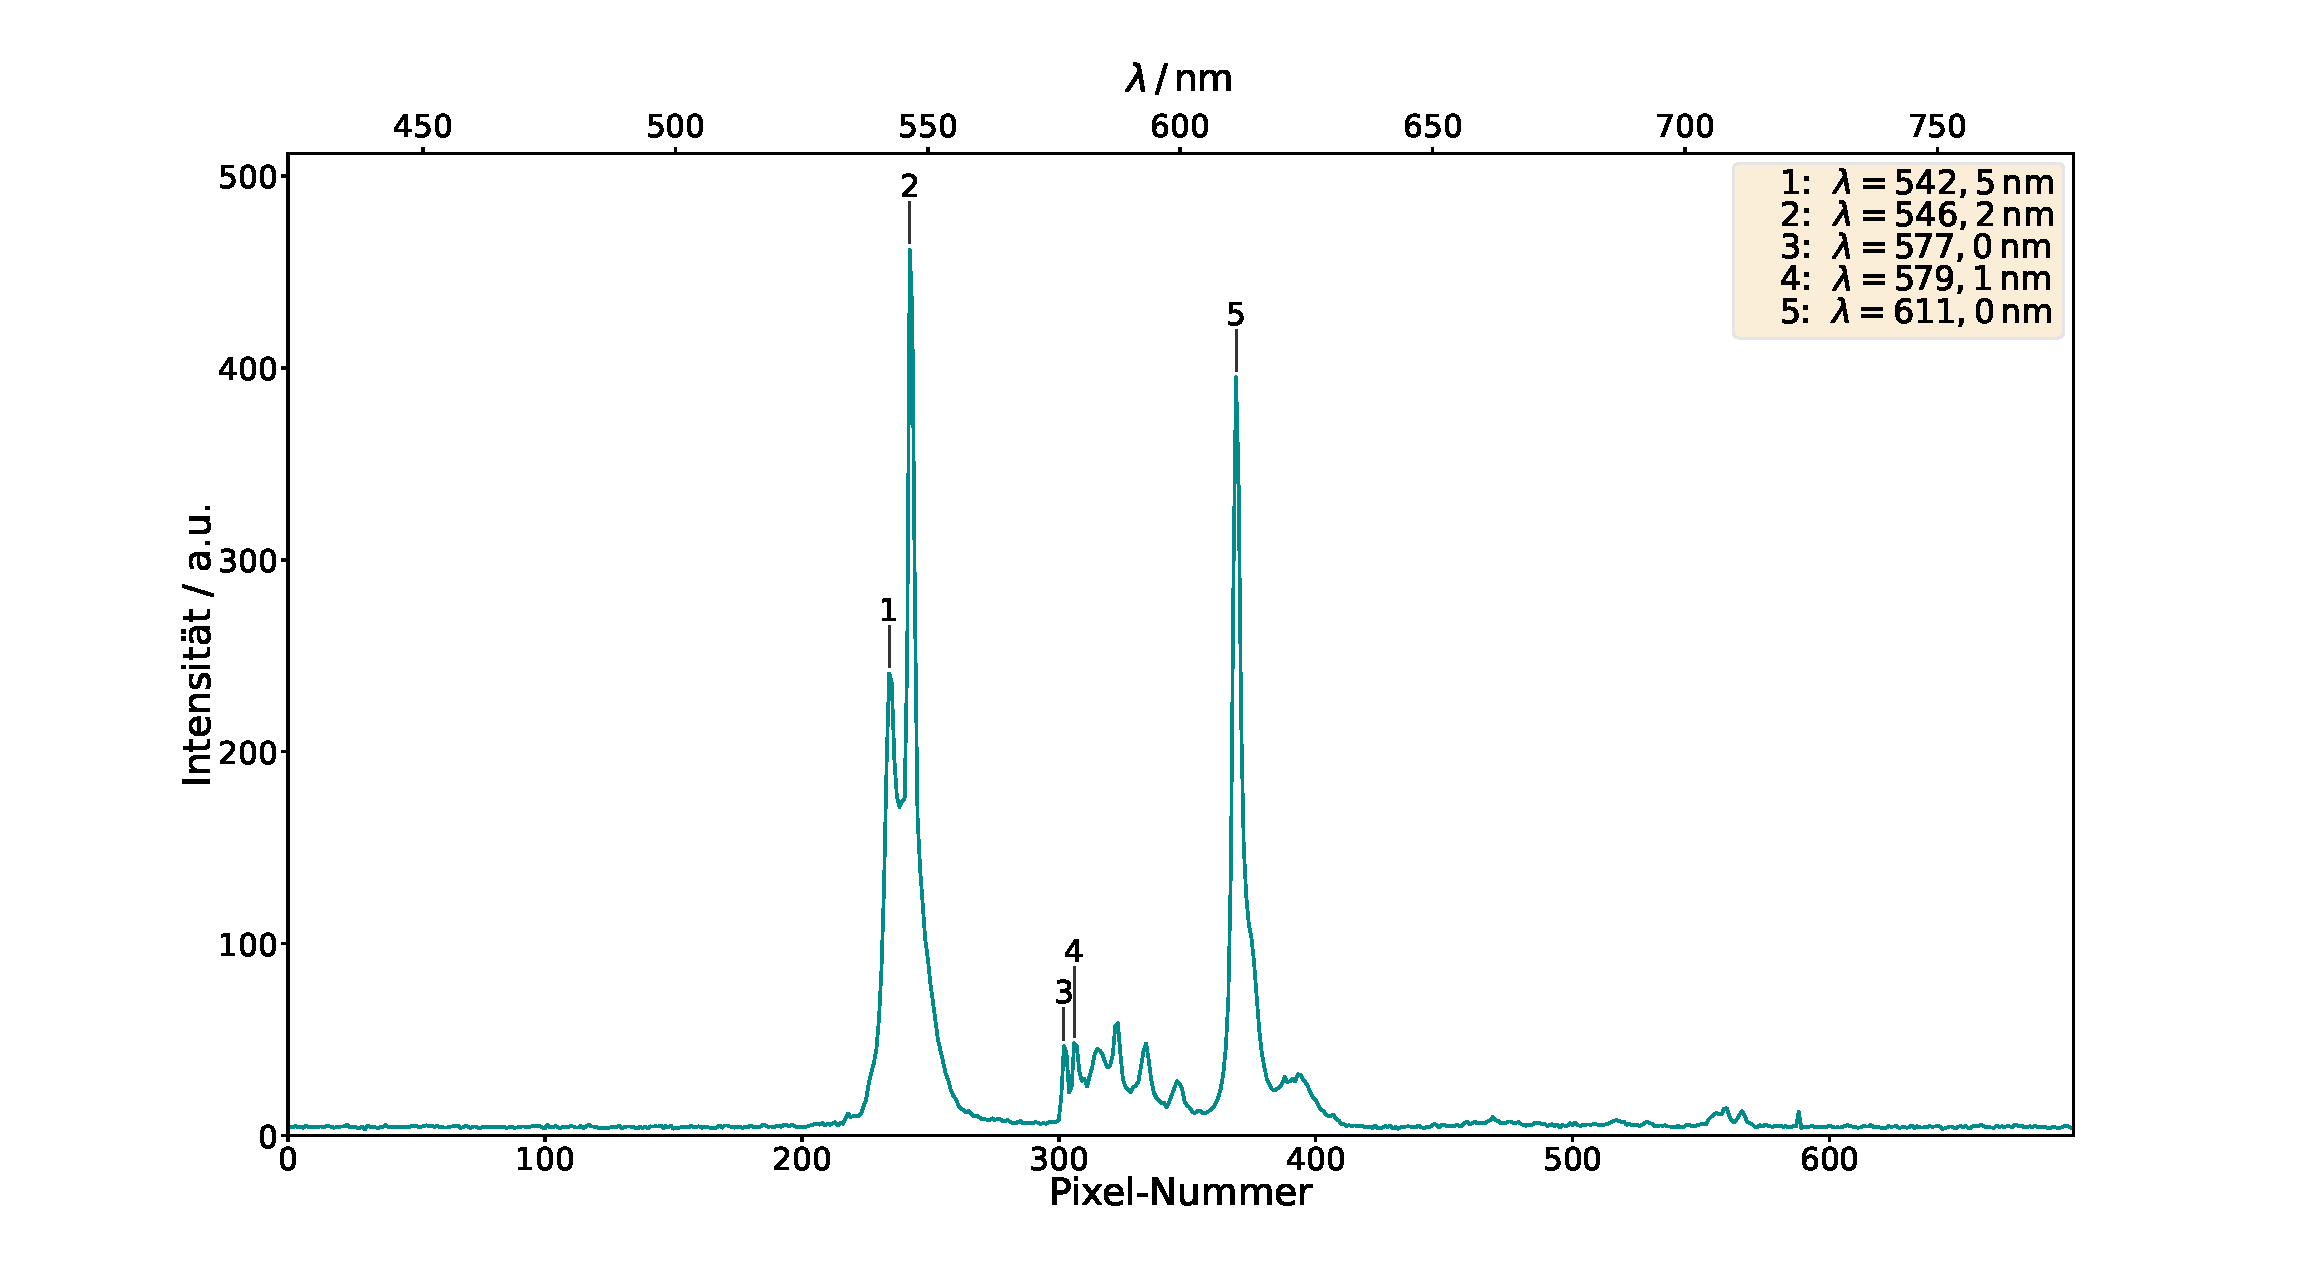
\includegraphics[clip, trim={3cm 1cm 3cm 2.5cm}, width=\textwidth]{Kalib.pdf}
    \caption{\label{fig:kali}Die gemessene Photonenanzahl als normierte Intensität gegen den 
    gemessenen Winkel $\Theta_{\text{mess}}$ aufgetragen. Zusätzlich sind die 
    beobachtbaren charakteristischen Linien eingezeichnet und identifiziert. 
    Der erste erkennbaren Peak (direkt neben 1) konnte nicht eindeutig identifiziert werden,
    weswegen dieser für weitere Berechnungen ignoriert wird.}
\end{figure}\FloatBarrier
\begin{figure}[h!]
    \centering
    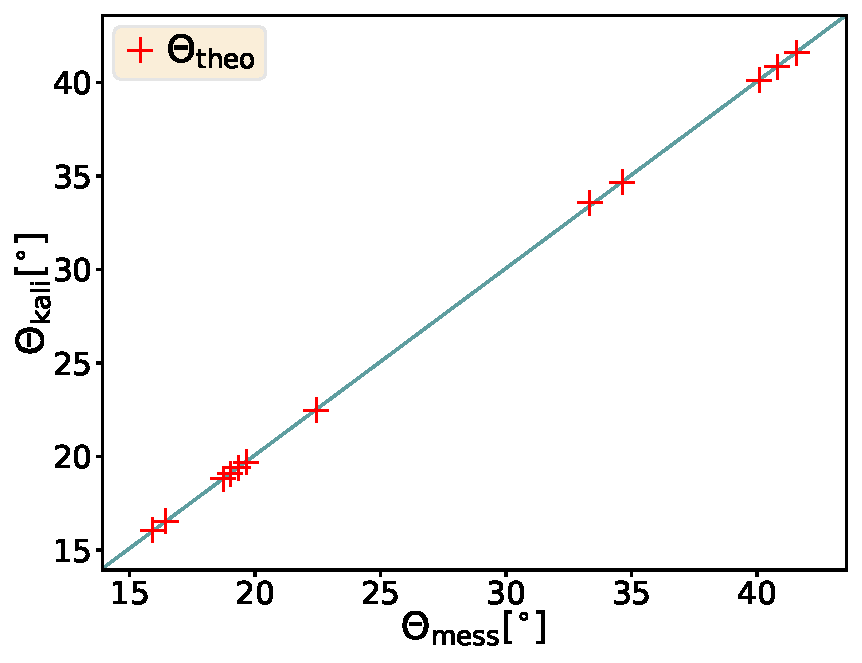
\includegraphics[width=0.6\textwidth]{fit.pdf}
    \caption{\label{fig:fitkali}Die theoretische Lage der identifizierten Linien gegen 
    die gemessene Lage aufgetragen. Zusätzlich ist eine Gerade zur Kalibration der gemessenen 
    Winkel durch die Werte gelegt. Aufgrund der Übersichtlichkeit wir nur der relevante 
    Bereich dargestellt, während der Achsenabschnitt im Haupttext dargestellt ist.}
\end{figure}\FloatBarrier
Aus dem errechneten Wert der Steigung kann man auf Linearität der Messgeräte schließen, da sie innerhalb 
des Fehlers die Identität bildet. Der Achsenabschnitt ist nicht vernachlässigbar, weist jedoch einen
hohen Fehler auf. \\
Die Korrektur des gemessenen Beugungswinkels wird trotz der erhaltenen Linearität 
mit beiden Werten durchgeführt, was unter 
Benutzung von Gl.~\eqref{eq:welle} zum gewünschten Spektrum führt. 
Zu beachten ist hierbei die Fehlerfortpflanzung des linearen Fits, was zu folgendem 
Fehler der Wellenlänge führt
\begin{align}
    s_{\lambda} &= \left\vert\frac{\partial \lambda}{\partial \Theta}\right\vert = \left\vert2d\cos(\Theta)s_{\Theta}\right\vert  \label{eq:errkali}\\
    s_{\Theta} &= \sqrt{\left(\Theta_{\text{kali}}s_{m}\right)^{2} + s_{b}^{2}}.
\end{align}
Dieser Wert muss bei der folgenden Kantenbestimmung zusätzlich zum Ablesefehler berücksichtigt werden. \\
\subsubsection{Identifizierung des Metallplättchens}
Nachdem die gemessenen Winkel richtig kalibriert und in Wellenlängen umgerechnet sind, können wir die 
gemessenen Spektren betrachten und hieraus das Material des Metallplättchens identifizieren. 
Die energetische Lage der K-Absorptionskante lässt sich mit folgender Formel für Elemente mit 
einer Ordnungszahl $Z>13$ annähern \cite{Kener}
\begin{equation}
    E_{K}/\si{eV} \approx 14\left(Z-3\right)^{2}.
\end{equation}
Außerdem lässt sich aus Vergleich der Datenbankwerte \cite{Database} direkt erkennen, dass 
das gesuchte Metall in der fünften Periode des Periodensystems zu suchen ist, da die K-Absorptionskante 
im Bereich von $\lambda\approx 0,5\,\si{\angstrom}$ liegt. \\
In Abb.~\ref{fig:metallspekt} sind die gemessenen Spektren als Funktion der kalibrierten 
Wellenlänge dargestellt.
\begin{figure}[h!]
    \centering
    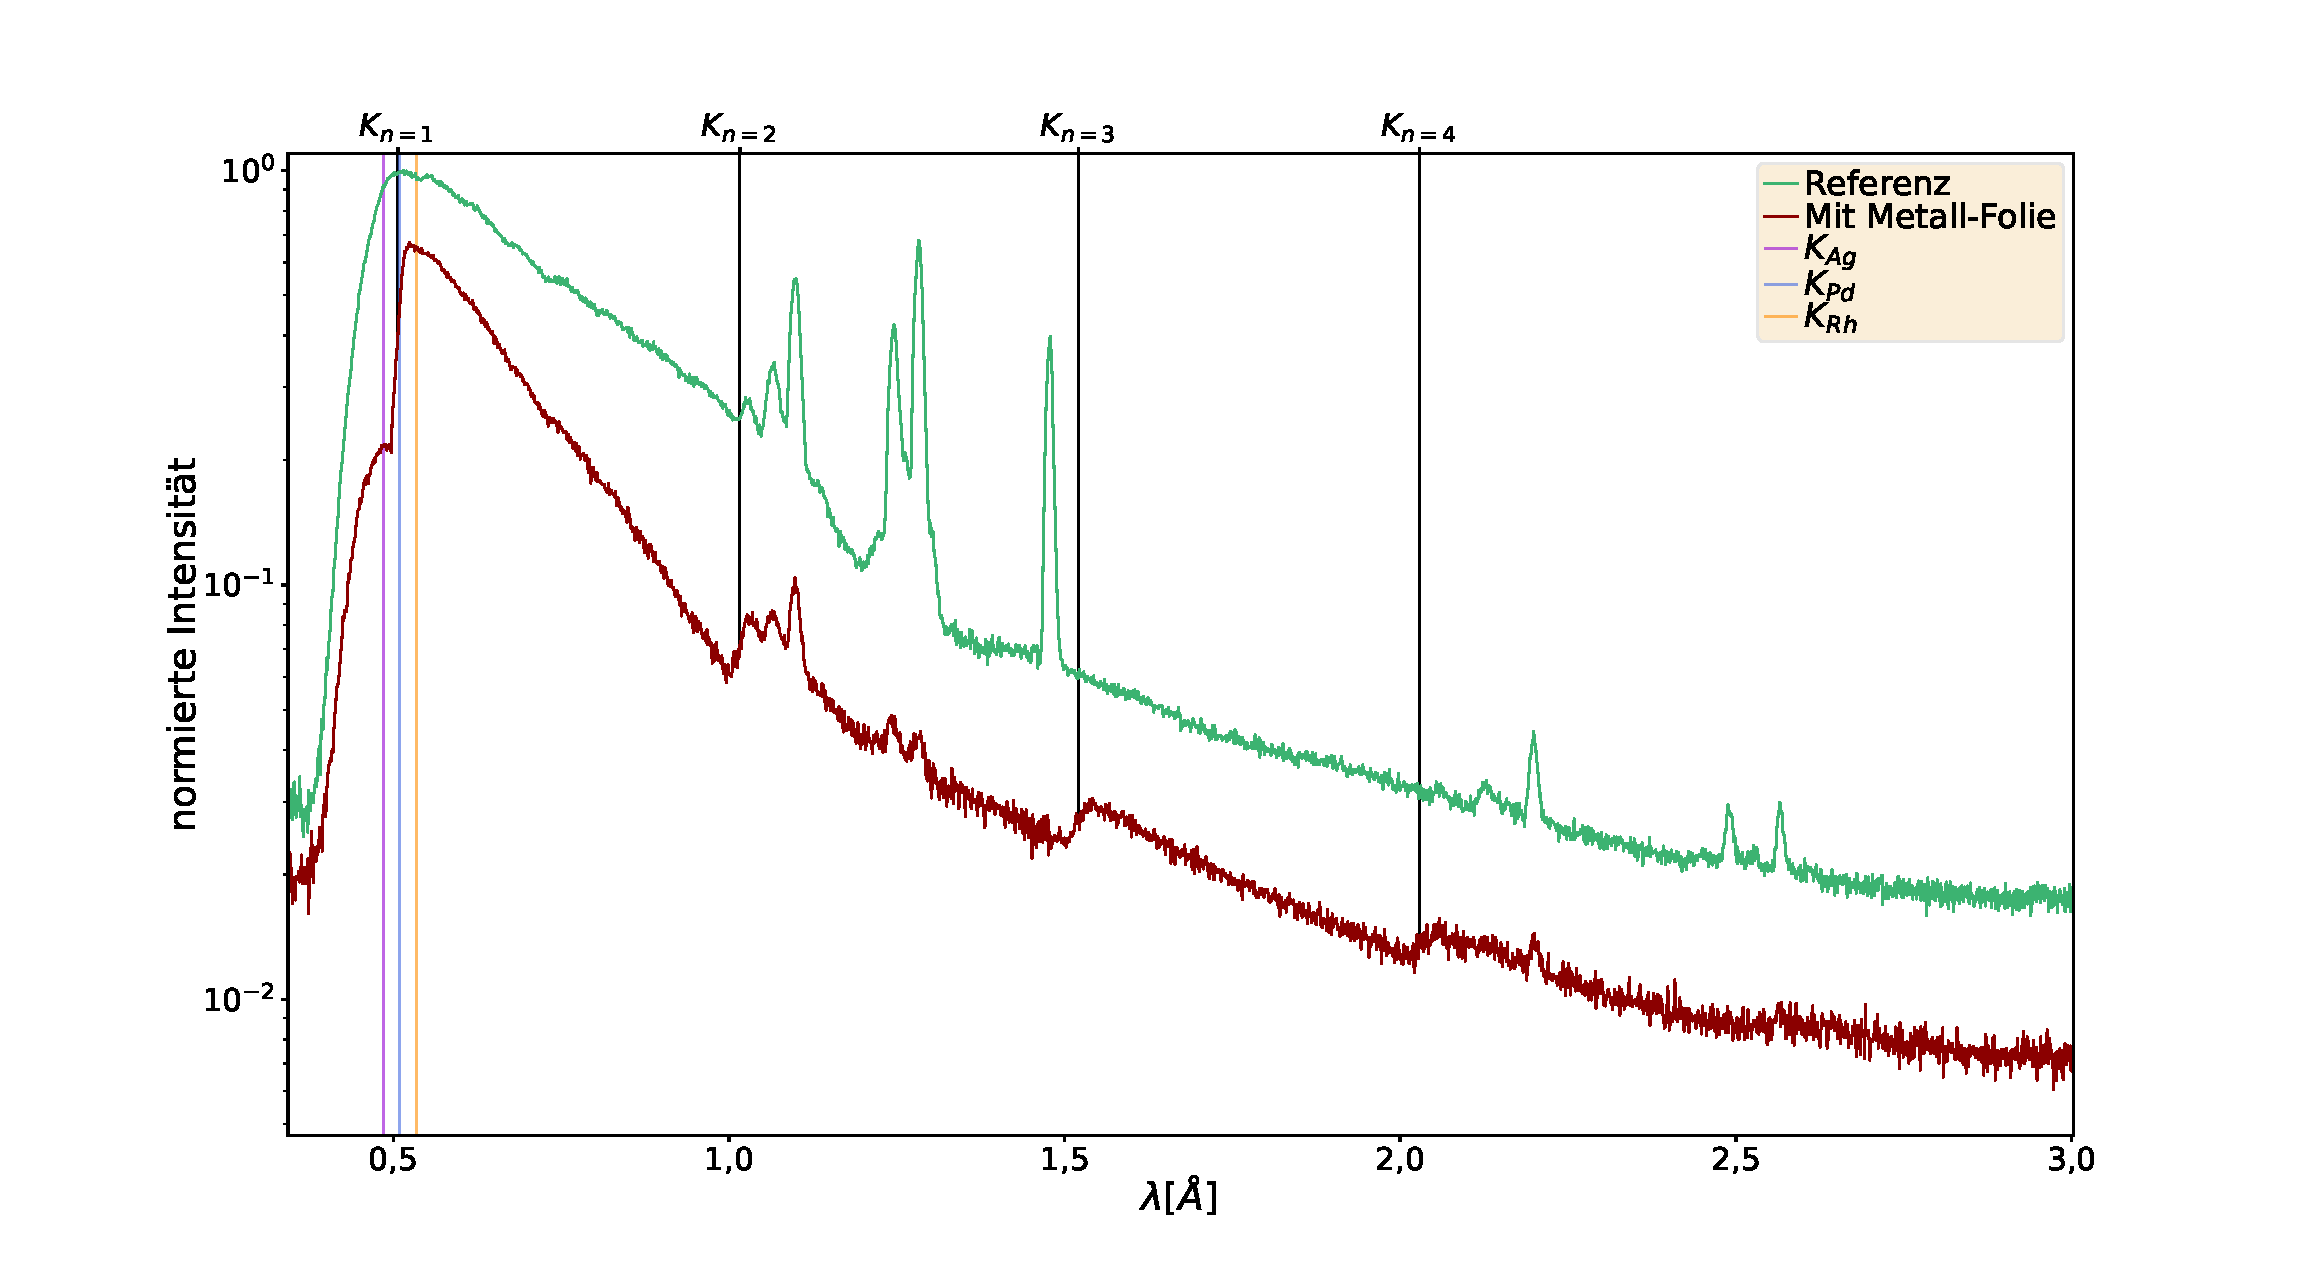
\includegraphics[clip, trim={2.7cm 1cm 3cm 2.5cm}, width=\textwidth]{Metall.pdf}
    \caption{\label{fig:metallspekt}Die gemessenen Spektren (Referenz und mit Metall-Folie)
    als Funktion der kalibrierten Wellenlänge. Die Intensität ist auf den maximalen Intensitätswert der 
    Referenz normiert und die y-Achse skaliert logarithmisch, um die Kanten besser erkennbare zu machen.
    Es sind die identifizierten K-Absorptionskanten aller auftretenden höherer Ordnungen, sowie die 
    Kanten von möglichen Metallen dargestellt.}
\end{figure}\FloatBarrier
Zur genauen Bestimmung der Lage der K-Kante, werden alle auftretenden 
Ordnungen berücksichtigt, um den Bestimmungsfehler zu minimieren.
Als Ablesefehler wählen wir $s_{\lambda,\text{ abl}} = n0,01\,\si{\angstrom}$, welcher sich aus
dem Auflösungsvermögen und der Beugungsordnung $n$ ergibt. Hierzu muss der Kalibrierungsfehler $s_{\lambda,\text{ kal}}$ 
aus Gl.~\eqref{eq:errkali} beachtet werden, sodass sich der gesamte Fehler der Wellenlängenbestimmung 
folglich ergibt
\begin{equation}\label{eq:fehler}
    s_{\lambda} = \sqrt{s_{\lambda,\text{ abl}}^{2} + s_{\lambda,\text{ kal}}^{2}}.
\end{equation} 
Die Lage der Absorptionskanten, sowie die zugehörigen Fehler ergeben sich zu
\begin{alignat}{2}  
    \lambda_{n=1} &= (0,5066\pm0,0106)\,\si{\angstrom}\hspace{2.5cm}\lambda_{n=2} &&= (1,0163\pm0,0204)\,\si{\angstrom} \\
    \lambda_{n=3} &= (1,5210\pm0,0303)\,\si{\angstrom}\hspace{2.5cm}\lambda_{n=4} &&= (2,0284\pm0,0403)\,\si{\angstrom},
\end{alignat}
woraus wir die Lage der K-Absorptionskante erster Ordnung bestimmen
\begin{align}
    \lambda_{K_{n=1}} &= (0,5072125\pm0,0102459)\,\si{\angstrom} \\
    \Rightarrow\Aboxed{\lambda_{K_{n=1}} &= (0,507\pm0,010)\,\si{\angstrom}}.
\end{align}
Betrachten wir die theoretische Lage der Absorptionskanten der infrage kommenden Metalle
\begin{equation}
    \lambda_{K_{\text{Ag}}} = 0,4859\,\si{\angstrom}\hspace{1cm}\lambda_{K_{\text{Pd}}} = 0,5092\,\si{\angstrom}\hspace{1cm}
    \lambda_{K_{\text{Rh}}} = 0,5340\,\si{\angstrom},
\end{equation} 
so bestätigt sich die optische Übereinstimmung aus Abb.~\ref{fig:metallspekt} mit Palladium (Pd).
Die Kanten für Rhodium (Rh) und Silber (Ag) liegen nicht im ersten Fehlerintervall, was zeigt, 
dass wir das Metall mit ausreichender Genauigkeit eindeutig identifizieren können. \\
Für das identifizierte Metall Palladium finden wir aus Ref.~\cite{Database} weiter L-Absorptionskanten, 
die jedoch außerhalb des gemessenen Bereichs liegen 
\begin{equation}
    L-I\rightarrow 3,4399\,\si{\angstrom}\hspace{1.5cm}
    L-II\rightarrow 3,7229\,\si{\angstrom}\hspace{1.5cm}
    L-III\rightarrow 3,9071\,\si{\angstrom}.
\end{equation}
Die Dichte von Palladium beträgt $\rho= 12,023\,\si{g/cm^{3}}$, was wir im 
folgenden Auswertungsschritt benötigen. \\
\subsubsection{K-Absorptionskante der ersten Ordnung}
Zur genauen und übersichtlichen Darstellung konzentrieren wir uns nur auf dem Bereich der ersten Absorptionskante
und stellen in diesem Bereich den Massenabsorptionskoeffizienten $\frac{\mu}{\rho}(\lambda)$ dar. 
Aus Gl.~\eqref{eq:massI} erhalten wir folgende Bestimmungsgleichung
\begin{equation}
    \frac{\mu}{\rho}(\lambda) = -\frac{1}{\rho x}\ln\left(\frac{I_{\text{Metall}}}{I_{\text{Ref}}}\right).
\end{equation}
In Abb.~\ref{fig:massI} ist ein kleiner Bereich des Massenabsorptionskoeffizienten 
um die K-Absorptionskante dargestellt.
\begin{figure}[h!]
    \centering
    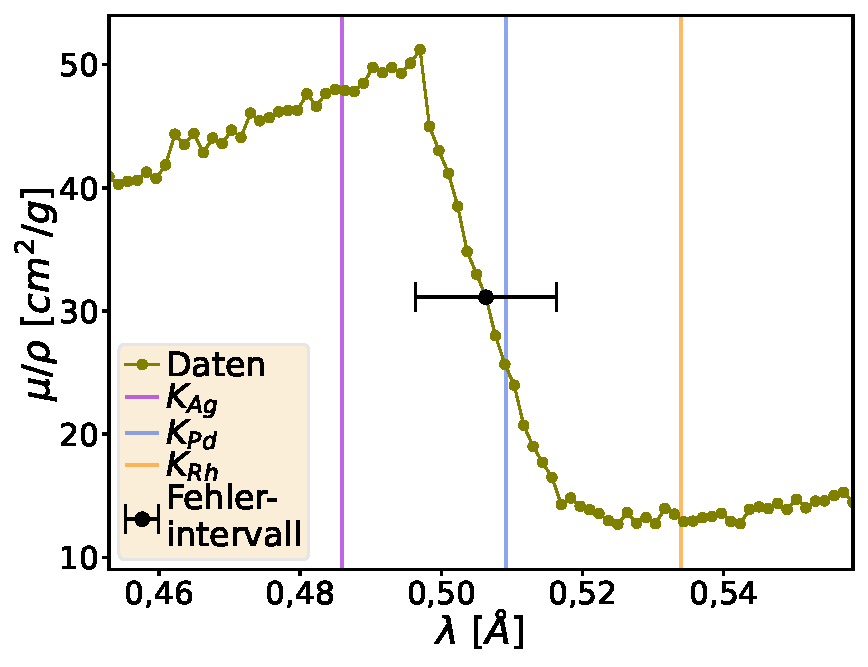
\includegraphics[width=0.5\textwidth]{massI.pdf}
    \caption{\label{fig:massI}Massenabsorptionskoeffizient $\mu/\rho$ als Funktion der Wellenlänge in einem 
    kleinen Intervall um die K-Absorptionskante. Zusätzlich sind die theoretischen 
    Lagen dieser Kanten für verschiedene Metall (Ag, Pd, Rh) eingezeichnet \cite{Database}. 
    Das Fehlerintervall ergibt sich aus Gl.~\eqref{eq:fehler}.}
\end{figure} \FloatBarrier
Es ist zu erkennen, dass die Lage der Absorptionskante innerhalb des ersten Fehlerintervalls 
mit der K-Kante von Palladium übereinstimmt, was aus der vorhergehenden Rechnung zu erwarten 
war. \\
Der Verlauf des Massenabsorptionskoeffizient lässt sich am besten in einer energetischen 
Betrachtung durchführen. Zur Ionisation von Elektronen aus der K-Schale wird eine 
gewisse Mindestenergie (Ionisierungsenergie) benötigt. Ist die Energie zu klein und damit 
die Wellenlänge zu groß, so ist die Absorption der Materie gering und nur durch andere 
Faktoren gegeben. Im Bereich der K-Kante steigt der Absorption schlagartig an, da hier 
die Energie zur Ionisation ausreicht und die Strahlung daher stärker mit der Materie wechselwirkt 
und somit Intensität raubt. Überschreitet man diese Energie und geht zu kürzeren Wellenlängen über,
so sinkt die Ionisationswahrscheinlichkeit, was sich aus Quantenmechanischen Überlegungen und 
der Diskretisierung der Energieniveaus ergibt. Der Massenabsorptionskoeffizient fällt daher 
in Richtung kürzerer Wellenlängen wieder ab. \\
\subsubsection{Beurteilung der Messung}
Insgesamt können wir aus den Messdaten eindeutig das absorbierende Metall identifizieren, was 
auf die Richtigkeit der Justage und der Durchführung deutet. 
Zur Bewertung des Messbereichs muss zunächst über Gl.~\eqref{eq:minlam} die minimal erreichbare 
Wellenlänge bzw.~maximale Energie der Röntgenstrahlung errechnet werden. Da wir bei einer Spannung 
von $U=50\,\si{kV}$ beträgt die minimal erreichbare Wellenlänge ungefähr 
$\lambda_{\text{min}}\approx0,25\,\si{\angstrom}$, was mit Gl.~\eqref{eq:winkel} einem Minimalwinkel 
von $\Theta_{\text{min}}\approx3,7^{\circ}$ entspricht. Der Messstart bei $\Theta_{0} = 5,0^{\circ}$ 
erscheint daher sinnvoll. Die maximal Wellenlänge bzw.~der Maximalwinkel bis zu welchem gemessen wird, 
ergibt sich aus dem Messaufbau und den verwendeten Geräten. Die Intensität der Röntgenstrahlung nimmt 
stark mit steigender Wellenlänge ab (vgl.~Abb.~\ref{fig:char}), wodurch das Signal 
bei gegebenen Untergrund schwer detektierbar wird. Anhand der gemessenen Spektren scheint der 
Maximalwinkel $\Theta_{\text{max}} = 51,0^{\circ}$ sinnvoll gewählt, da im hinteren Bereich der 
Messung eine Unterscheidung vom Untergrund nicht mehr funktioniert. \\
Will man auch in einem Winkelbereich schwacher Röntgenintensität aussagekräftige Messungen 
durchführen, so muss die Integrationszeit weiter erhöht werden. Für das Praktikum sind die 
Integrationszeiten sinnvoll, da hierdurch bei übersichtlicher Messdauer dennoch ein 
gut entwickeltes Signal gemessen wird. \\
Die Winkelschrittweite von $\Delta{\Theta} = 0,02^{\circ}$ resultiert in einer maximalen Wellenlängenänderung 
von $\Delta{\lambda}_{\text{max}}\approx 0,0013\,\si{\angstrom}$. Hiermit lassen sich Änderungen, und Peaks 
sehr genau einschränken, was die Schrittweite legitimiert. Je nach Anwendung können diese Parameter eingestellt
werden, um schnelle oder genaue Ergebnisse zu erhalten. \\
Um die $K\alpha$-Linien sinnvoll zu messen, muss zunächst die Energie der Röntgenstrahlung ausreichen, um 
die benötigte Ionisation zu erreichen. Rechnerisch ergibt sich aus Gl.~\eqref{eq:winkel} eine benötigte 
Spannung von $U>59,3\,\si{kV}$. Da die Bremsstrahlung die charakteristische Strahlung überdecken kann, 
solle eine deutlich größere Spannung gewählt werden, um die Peaks getrennt vom restlichen Signal aufzulösen. \\
Zusammenfassend war die Messung erfolgreich und die Ergebnisse im erwarteten Rahmen. Der zeitliche 
Aufwand der Messung ist vertretbar und die Einstellung der Messgeräte interessant. Im folgenden Abschnitt
analysieren wir die Ergebnisse des zweiten Versuchteils. \\








